\documentclass[aspectratio=169]{beamer}

\usetheme{default}
\setbeamertemplate{navigation symbols}{}
\setbeamertemplate{enumerate item}{\color{navy}\arabic{enumi}.}
\setbeamertemplate{itemize item}{\color{black}\textbullet}
\setbeamertemplate{itemize subitem}{\color{black}\textbullet}
\usepackage{booktabs}
\usepackage{xcolor}
\usepackage{tikz}
\usetikzlibrary{shapes,arrows,positioning}
\definecolor{navy}{RGB}{0, 0, 128}
\definecolor{lightblue}{RGB}{230,240,250}
\definecolor{darkgreen}{RGB}{0,100,0}
\definecolor{lightgreen}{RGB}{230,250,230}
\newcommand{\highlight}[1]{\colorbox{lightblue}{$\displaystyle\textcolor{navy}{#1}$}}
\newcommand{\highlighttext}[1]{\colorbox{lightblue}{\textcolor{navy}{#1}}}
\newcommand{\highlightgreen}[1]{\colorbox{lightgreen}{$\displaystyle\textcolor{darkgreen}{#1}$}}

\usepackage{hyperref}
\hypersetup{
    colorlinks=true,
    linkcolor=navy,
    urlcolor=navy,
    citecolor=navy
}

\begin{document}

\begin{frame}
\centering

\includegraphics[width=0.4\textwidth]{Heckman_Stixrud_Urzua_2006_JOLE_cover.jpg}
\end{frame}

\begin{frame}

\textcolor{navy}{Core Structure:} Factor model with two latent abilities ($f^C, f^N$)

\bigskip

\onslide<2->{
$$
Y_{s} = \beta_{Y,s} X_Y + \alpha^C_{Y,s} f^C + \alpha^N_{Y,s} f^N + e_{Y,s}
$$
}

\bigskip

\onslide<3->{
\textcolor{navy}{Key features:}
\bigskip

\begin{itemize}
\itemsep1.5em
\item<4-> Loadings vary by $s$; factors explain all dependence
\end{itemize}
}

\end{frame}

\begin{frame}

\onslide<1->{
The model covers:
\bigskip
}

\begin{itemize}
\itemsep1.5em
\item<2-> Wages, employment, occupation, work experience
\item<3-> Schooling choice
\item<4-> Risky behaviors (smoking, drugs, crime, pregnancy)
\end{itemize}

\end{frame}



\begin{frame}

\onslide<1->{
A life cycle model provides economic interpretation
}

\bigskip

\onslide<2->{
Maximize:
$$
\int_0^T \exp(-\rho t) U(c(t), l(t); \eta) dt
$$
}

\bigskip

\onslide<3->{
Subject to:
\bigskip
}

\begin{itemize}
\itemsep1.5em
\item<4-> Human capital production: $\dot{h}(t) = \varphi(h(t), I(t); \tau)$
\item<5-> Wage equation: $Y(t) = R(h(t); \theta)$
\item<6-> Budget constraint: $\dot{A}(t) = Y(t)h(t)l(t) - P(t)'c(t) + rA(t)$
\end{itemize}

\end{frame}



\begin{frame}
Why do we need an economic model?
\bigskip

\begin{itemize}
\itemsep1.5em
\item<2-> \textcolor{navy}{Interpretation:} Statistical model is just linear approximation
\item<3-> \textcolor{navy}{Microfoundations:} Economic model provides structural meaning to factors
\item<4-> \textcolor{navy}{Mechanisms:} Shows \emph{how} abilities operate (preferences vs productivity, etc.)
\item<5-> \textcolor{navy}{Policy relevance:} (Could) simulate effects of interventions on primitives
\end{itemize}

\end{frame}

\begin{frame}
Identification:
\bigskip\par
\begin{itemize}
\itemsep1.5em
    \item<2-> Identification mainly through exclusion restrictions \& variation in measurements
    \item<3-> Variation allows for separation of two factors and different effects on outcomes
\end{itemize}
\bigskip

\onslide<4->{
Estimation:
\bigskip\par
}
\begin{itemize}
\itemsep1.5em
    \item<5-> Use MCMC to estimate parameters of the statistical model
\end{itemize}
\bigskip

\onslide<6->{
Simulations:
\bigskip\par
}
\begin{itemize}
\itemsep1.5em
    \item<7-> Simulate model to plot conditional expectations of outcomes given factors
    \item<8-> Find evidence that the 2 factors do indeed load onto all outcomes
\end{itemize}

\end{frame}


\begin{frame}
\centering
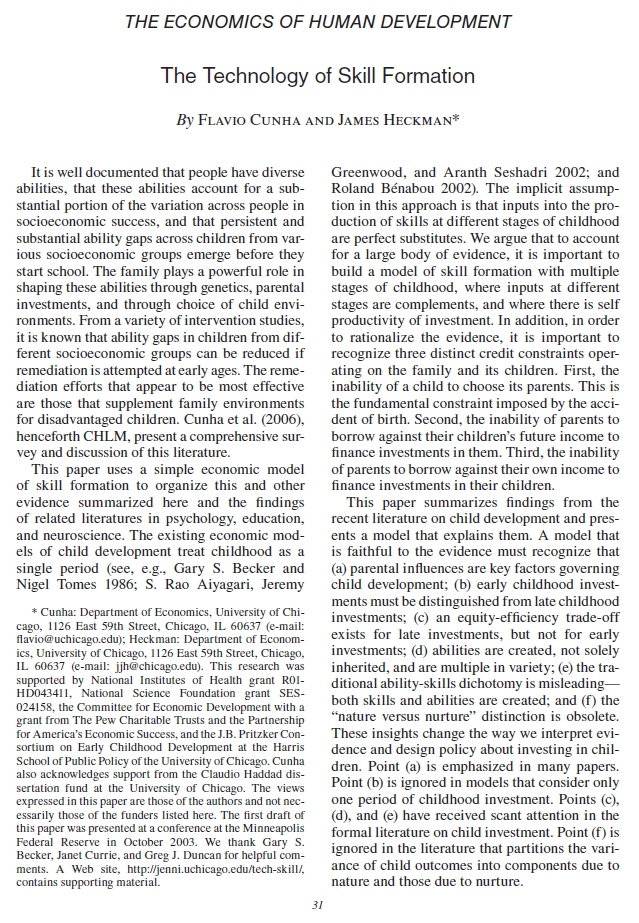
\includegraphics[width=0.4\textwidth]{Cunha_Heckman_2007_AER_cover.jpg}
\end{frame}

\begin{frame}
Skills are produced through multi-stage process given investment $I_t$:
\bigskip

\begin{itemize}
\itemsep1.5em
\item<2-> Self-productivity: $\theta_{t+1} = f_t(\theta_t, I_t)$ 
\item<3-> Dynamic complementarity: Early and late investments complement each other
\item<4-> Critical periods: Early gaps persist; early intervention most effective
\end{itemize}

\bigskip
\onslide<5->{
\textcolor{navy}{Policy implication:} No equity-efficiency tradeoff for early childhood investment
}
\end{frame}

\begin{frame}
\centering
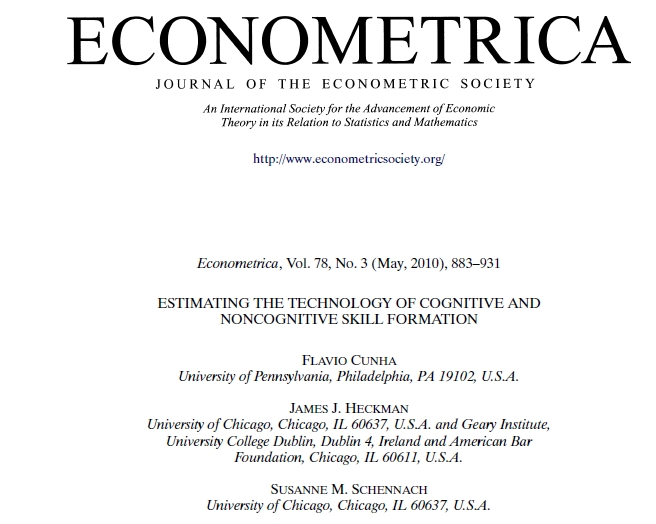
\includegraphics[width=0.6\textwidth]{CHS_2010_Econometrica_cover.jpg}
\end{frame}

\begin{frame}
\textcolor{navy}{Contribution:} Nonparametric identification and estimation of the technology
\bigskip

\begin{itemize}
\itemsep1.5em
\item<2-> Identifies elasticity of substitution between $\theta_t$ and $I_t$
\item<3-> Accounts for endogeneity of parental investments
\item<4-> Anchors test scores to avoid arbitrary scaling
\end{itemize}

\onslide<5->{
\bigskip
\textcolor{navy}{Key finding:} Substitutability decreases over life cycle for cognitive skills (early investment crucial); constant for noncognitive skills
}
\end{frame}


\end{document}